By {\it Rate Curves Framework} we mean a set of Excel spreadsheets which execute multi-curve calibration for the main currencies. So far, the framework includes 30 rate curves for 7 currencies (see Table \ref{tab:1}) as well as a Standard Curve for each currency. 

\begin{table}[]
\centering
\begin{tabular}{|l||c|c|c|c|c|c|}
 \hline
 Currency/Tenor & ON & 1M & 3M & 6M & 1Y \\
 \hline \hline
 EUR & \checkmark & \checkmark & \checkmark & \checkmark & \checkmark\\
 \hline
 GBP & \checkmark & \checkmark & \checkmark & \checkmark & \checkmark\\
 \hline
 USD & \checkmark & \checkmark & \checkmark & \checkmark & \checkmark\\
 \hline
 HKD & \checkmark & \checkmark & \checkmark & \checkmark & \\
 \hline
 JPY & \checkmark & & \checkmark & \checkmark & \\
 \hline
 AUD & \checkmark & \checkmark & \checkmark & \checkmark & \\
 \hline
 SEK & \checkmark & \checkmark & \checkmark & \checkmark & \\
 \hline
 \end{tabular}
\caption{The 30 curves of Rate Curves Framework}
\label{tab:1}
\end{table}

A Rate Curve, or Term Structure of Interest Rates, could be defined as the relationship between discount factors and times but we will see that this is only one of the possible definitions. For each currency-tenor pair, curve calibration is the process which computes this term structure starting from a set of liquid Interest Rate Derivatives with different maturities whose quotes are available on the market. By quote we mean any number that is used by the market to indicate the level of a financial instrument: rate, price, yield, and so on. Even if there are a lot of liquid instruments, we don't have an instrument for each maturity date. This is the reason way an "interpolation" method has to be used to obtain the entire curve. All these modelling issues will be analyzed in Chapter \ref{chap:2}. Chapter \ref{chap:4}, instead, describes a concrete example, the EUR market case, in order to produce a new proposal for the EUR Rate Curve Framework. 

This introduction aims to briefly describe why this framework exist and how it has been integrated into the existing infrastructure.

The framework was born after 2007 crisis in order to integrate official systems with new functionalities (e.i. multi-curve and exogenous ois discounting) which at that time were not supported yet. Today the implementation of new curve construction models inside front office systems is still a problem and is one of the reason why the Excel framework exists: it is more flexible and allows faster changes.

Another reason is that our systems are not able to pre-process any market information before calibration. In other words the input of the calibration process inside the system must be a market quote. In general manipulation of market quotes is not recommended (see \cite{henrard} for more details) but in some cases we are forced to create "synthetic quotes", not available but derivable from market�s information. The corresponding instruments are named {\it synthetic instruments}. The Excel Framework plays a fundamental role here because it can calculate these synthetic quotes and send them to legacy systems as market quotes.

The starting point is {\it Thomson Reuters Eikon Platform}, where all market quotes are published on the so called "External Channel". Each market quote is identified by a specific code, named RIC ({\it Reuters Identification Code}). In order to make these quotes available on Excel interface, a specific Excel Add-In has been developed by Thomson Reuters (by Add-in we mean a specific type of application used to add features to Excel). This Add-In allows the real time download of market quotes from Thomson Reuters Eikon Platform to Microsoft Excel. These quotes are the input of the calibration process, which is performed thanks to {\it QuantLib} analytics.

QuantLib is a C++ free/open-source library for quantitative finance based on an object-oriented programming; it implements all the basic classes and methods used for calibration (bootstrapping algorithm, interpolations, market conventions). QuantLib functionality is exported to Microsoft Excel through QuantLibXL Add-In. For more information please visit {\it quantlib.org}.

Once the curve has been calibrated, the main issue is how to export the related information from Excel to the front office systems, which expect as input a set of market quotes (as discussed). The solution is to define a new set of instruments (which may also include different type of synthetic instruments) and price them using the calibrated curve obtaining new quotes. Obviously all the instruments used for calibration must be "at market level" when priced by the calibrated curve. Each new quote is identified by a new code, published on Eikon Internal Channel (available only for bank internal users) and used to perform a second calibration inside the system.

The key point of this {\it contribution process} is that the system calibration could use a set of instruments totally different from the one used for the Excel calibration. Also, the two calibrations could be different not only for the selected instruments but also for a different choice of settings (interpolation, start date,...). For the EUR market case, these differences will be justified in Chapter \ref{chap:4}.

Figure \ref{fig:1} represents the whole infrastructure.

\begin{figure}
\centering
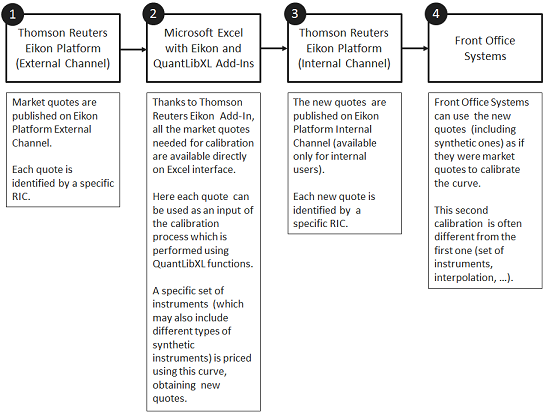
\includegraphics{images/1.png}
\caption{Rate Curves Infrastructure}
\label{fig:1}
\end{figure}





 











 
